% This syllabus template was created by:
% Brian R. Hall
% Assistant Professor, Champlain College
% www.brianrhall.net

% Document settings
\documentclass[11pt]{article}
\usepackage[margin=1in]{geometry}
\usepackage[pdftex]{graphicx}
\usepackage{multirow}
\usepackage{setspace}
\usepackage{listings}
\pagestyle{plain}
\setlength\parindent{0pt}

\begin{document}
	
	\section*{Mécanique des fluides : statique}
	
	Un fluide est un milieu qui ne résiste pas aux forces de cisaillement et qui prend la forme de son récipient. On distingue les gaz, dont le volume est variable, et les liquides, dont le volume est (quasi) constant dans des conditions normales.
	
	\subsection*{Pression dans un fluide}
	
	La force exercée par un liquide au repos sur une petite surface plane est égale à la pression multipliée par la surface :
	\[
	\vec{F} = P \, \vec{S}
	\]
	
	La force est un vecteur, tandis que la pression est une grandeur scalaire. La surface est ici considérée comme une surface orientée.
	
	En un point donné d’un fluide au repos,   {la pression est la même dans toutes les directions}.
	
	\subsection*{Unité de pression}
	
	L’unité de pression dans le système international est le pascal (Pa), avec :
	\[
	1 \  \texttt{Pa} = 1 \  \texttt{N/m}^2
	\]
	
	\subsection*{Condition d’équilibre}
	
	Dans un fluide au repos, les forces se compensent en tout point : le fluide est en équilibre statique.
	
	\subsection*{Loi de Pascal}
	
	\newpage
	
	\subsection*{Loi de Pascal et ses applications}
	
	Toute variation de pression en un point d’un liquide contenu dans un récipient se transmet intégralement à tout le fluide.
	
	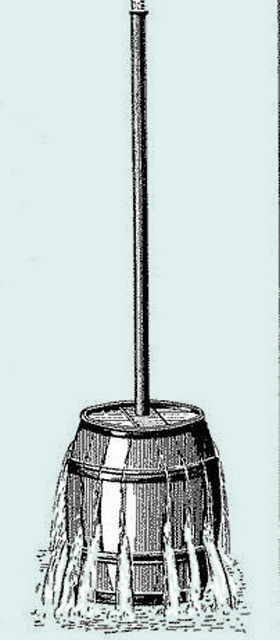
\includegraphics[width=0.5\linewidth]{images/tonneau.jpg}
	
	\subsection*{Loi fondamentale de la statique des fluides}
	
	\[
	P = \rho g h + P_0
	\]
	
	\subsection*{La loi d’Archimède comme conséquence de la loi fondamentale}
	
	La poussée d’Archimède résulte de la variation de la pression avec la profondeur dans un fluide.
	
	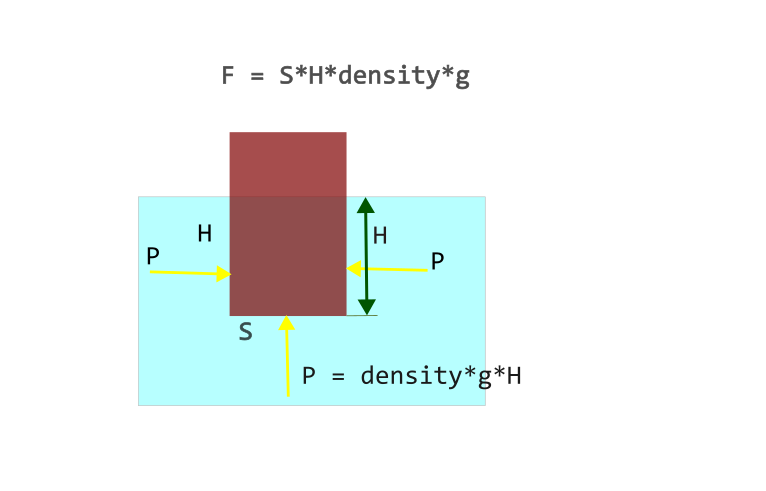
\includegraphics[width=0.5\linewidth]{images/archimed1.png}
	
	Elle peut être aussi expliquée par ce raisonnement: on remplace la partie immergée de l'objet par le liquide:
	
	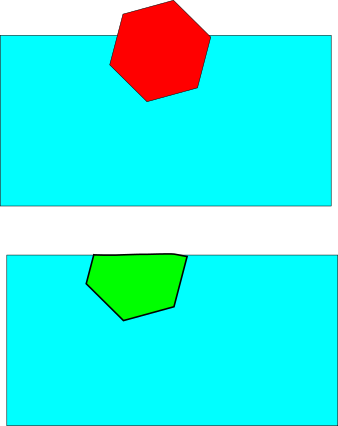
\includegraphics[width=0.2\linewidth]{images/archimed.png}
	
		\begin{equation}
		F_{arch} = {V_{immergee}} \times \rho \times g
	\end{equation}
	\subsection*{Tension superficielle}
	
	Il existe une expérience : une aiguille en acier peut flotter à la surface de l’eau. Or, l’acier est plus dense que l’eau, et la loi d’Archimède ne peut pas expliquer cet effet.
	
	Il existe donc une force à la surface de l’eau appelée   {tension superficielle}.
	
	Cette force s’oppose à l’augmentation de la surface de l’eau. On dit que la surface de l’eau possède une énergie superficielle.
	Cette force explique aussi la montée ou la descente de l'eau dans le capillaires selon la loi de Jurin:
	\begin{equation}
		h = \frac{2\gamma \cos\theta}{\rho g r}
	\end{equation}
	LA valeur $\gamma$ est appelée a tension superficielle du liquide, 
	\section*{Mécanique des fluides : dynamique}
	
	\subsection*{Débit}
	
	Le débit volumique est le volume de fluide qui traverse une section donnée en une seconde. Il est mesuré en $m^3/s$.
	
	Pour la vitesse $v$ et la surface $S$ :
	\[
	q_v = v \times S
	\]
	
	Le débit massique est la masse de fluide qui traverse une section donnée en une seconde. Il est mesuré en $kg/s$.
	
	Pour la vitesse $v$, la surface $S$ et la masse volumique $\rho$ :
	\[
	q_m = v \times S \times \rho
	\]
	
	En raison de la conservation de la masse, le débit massique est constant en écoulement stationnaire. C’est l’équation de continuité :
	\[
	q_m = v \times S \times \rho =  \texttt{constante}
	\]
	
	Si le fluide est incompressible (sa densité est constante), le débit volumique est aussi constant :
	\[
	q_v = v \times S =  \texttt{constante}
	\]
	
	Plus la section est petite, plus la vitesse d’écoulement est grande.
	
	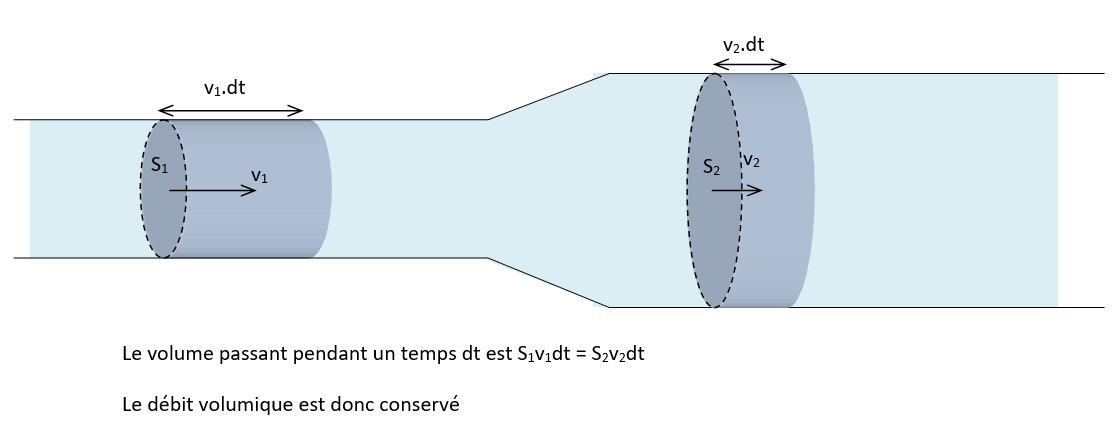
\includegraphics[width=0.5\linewidth]{images/ConservMasse.png}
	
	\subsection*{Loi de Bernoulli et pertes de charge}
	
	Comment la pression change-t-elle dans les tuyaux ? Il y a deux facteurs : le changement de section (donc de vitesse) et les frottements dans les tuyaux.
	
	La loi de Bernoulli est une conséquence de la conservation de l’énergie :
	\[
	P + \frac{1}{2}\rho v^2 =  \texttt{constante}
	\]
	
	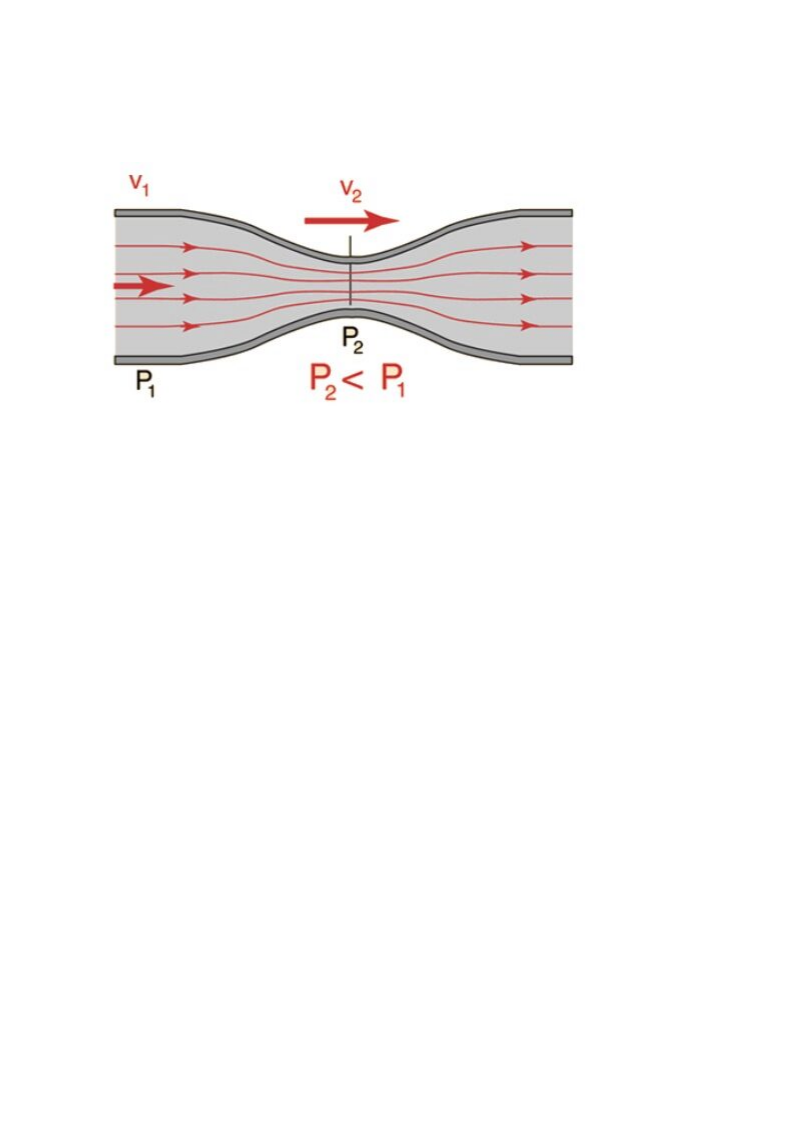
\includegraphics[width=0.5\linewidth]{images/bernulli.png}
	
\end{document}